
\section {Paragraf autorstwa Piotra Bieszczada}
Czym jest liczba \textbf{"e"} w matematyce ?
\\
Liczba \textbf{"e"} jest podstawą logarytmu naturalnego. Nazywa się ją liczbą \textbf{Eulera}. Jest ona wykorzystywana w wielu dziedzinach matematyki i fizyki. W przybliżeniu wynosi:\underline{2,718281828459[1].}
\\
\\
\textbf{Jest ona określana przez granicę następującego ciągu:}
    \begin{equation} \label{eq:1}
        \lim_{n \to \infty }\left({1+\frac{1}{n}}\right)^n=e
    \end{equation}
\textbf{Przy rozwiązywaniu zadań może nam się przydać taki wzór:}
    \begin{equation} \label{eq:2}
        \lim_{n \to \infty }\left({1+\frac{a}{n}}\right)^n=e^a
    \end{equation}
\textbf{Przykładowe rozwiązanie granicy ciągu z liczbą eulera:}
    \begin{equation} \label{eq:3}
        \lim_{n \to \infty }\left({1+\frac{6}{(n-1)}}\right)^{(n-1)}=e^6
    \end{equation}
\textbf{Ciekawostka :3} Całka z liczby \textbf{eulera} podniesionej do potęgi \textbf{x} wynosi:
    \begin{equation} \label{ex:4}
       \int{e^x}dx={e^x}+C
    \end{equation}
\underline{Tak dokładnie, wynosi tyle samo !}
\\
\\
Każdy student wie ,że \textbf{Leonhard Euler} to wybitny matematyk :)
\begin{figure}[htbp]
    \centering
    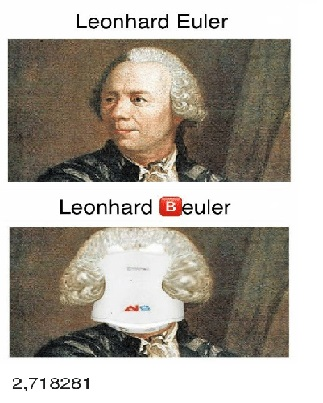
\includegraphics{pictures/leonhar_euler.jpg}
    \caption{Troszkę matematycznego humoru :)}
    \label{fig:my_label}
\end{figure}
\subsection{Formatowanie tekstu}
\textbf{Lorem ipsum} \textit{dolor sit amet, consectetur adipiscing elit, sed do eiusmod tempor incididunt ut labore et dolore magna aliqua. Ut enim ad minim veniam, quis nostrud exercitation ullamco laboris nisi ut aliquip ex ea commodo consequat.}
\\
\\
\\
\subsection{Formatowanie Tabeli}
Tabela~\ref{tab:agh} pokazuje progi punktowe na AGH w poszczególnych latach.


\begin{table} [htbp]
\centering
\begin{tabular}{|c|c|c|c|}
\hline
\rowcolor[HTML]{FE0000} 
{\color[HTML]{000000} Progi punktowe AGH}           & {\color[HTML]{000000} ISI} & {\color[HTML]{000000} INF} & {\color[HTML]{000000} AIR} \\ \hline
\rowcolor[HTML]{656565} 
\cellcolor[HTML]{009901}{\color[HTML]{000000} 2022} & {\color[HTML]{000000} 980} & {\color[HTML]{000000} 960} & {\color[HTML]{000000} 920} \\ \hline
\rowcolor[HTML]{656565} 
\cellcolor[HTML]{009901}{\color[HTML]{000000} 2021} & {\color[HTML]{000000} 970} & {\color[HTML]{000000} 980} & {\color[HTML]{000000} 910} \\ \hline
\rowcolor[HTML]{656565} 
\cellcolor[HTML]{009901}{\color[HTML]{000000} 2020} & {\color[HTML]{000000} 965} & {\color[HTML]{000000} 955} & {\color[HTML]{000000} 915} \\ \hline
\end{tabular}
\label{tab:agh}
\caption{Progi punktowe AGH.}
\end{table}


\subsection{Formatowanie nienumerowane}

\begin{itemize}
  \item Nienumerowane1
  \item Nienumerowane2
  \item Nienumerowane3
\end{itemize}

\subsection{Formatowanie numerowane}
\begin{enumerate}
    \item numerowane1
    \item numerowane2
    \item numerowane3
\end{enumerate}
